%!TEX TS-program =  pdflatex 


\documentclass{amsart}
\usepackage{array}
\newcolumntype{P}[1]{>{\raggedright\let\newline\\\arraybackslash\hspace{0pt}}m{#1}}
\usepackage{graphicx,verbatim, amsmath, amssymb, amsthm, amsfonts, epsfig, amsxtra,ifthen,mathtools,epstopdf,caption,enumerate,hyperref,hhline,bbm,capt-of,longtable}	
\DeclareFontFamily{U}{mathx}{\hyphenchar\font45}
\DeclareFontShape{U}{mathx}{m}{n}{<-> mathx10}{}
\DeclareSymbolFont{mathx}{U}{mathx}{m}{n}
\DeclareMathAccent{\widebar}{0}{mathx}{"73}
\epstopdfsetup{suffix=}
\DeclareGraphicsExtensions{.ps}
\DeclareGraphicsRule{.ps}{pdf}{.pdf}{`ps2pdf -dEPSCrop -dNOSAFER #1 \noexpand\OutputFile}

\newtheorem{proposition}{Proposition}[section]
\newtheorem{theorem}[proposition]{Theorem}
\newtheorem{corollary}[proposition]{Corollary}
\newtheorem{lemma}[proposition]{Lemma}
\newtheorem{prop}[proposition]{Proposition}
\newtheorem{cor}[proposition]{Corollary}
\newtheorem{thm}[proposition]{Theorem}
\newtheorem{conj}[proposition]{Conjecture}
\newtheorem{phen}{Phenomenon}

\renewcommand\thephen{\Roman{phen}}

\theoremstyle{definition}
\newtheorem{example}[proposition]{Example}
\newtheorem{definition}[proposition]{Definition}
\newtheorem{question}[proposition]{Question}

\theoremstyle{remark}
\newtheorem{remark}[proposition]{Remark}
\newtheorem{problem}[proposition]{Problem}

\numberwithin{equation}{section}
\usepackage[usenames]{color}

% commands for marginal notes below
% to make a marginal note, insert
% \margin{Your comment here.} in the text.
%  To sign the note:
% \margin[You]{Your comment here.}
% You can also label your comments and get a reference to the 
% number later, like:
% \margin[You]{Your comment here. \label{thefrivolouscomment}}
% Things may start to look ugly if you have more than 99 
%  marginal notes, but utility, not beauty is the intention here.
%  This uses the command \marginpar
%  defined, I think, in verbatim
%  The circled numbers will screw up the formatting slightly.

% Sometimes, if you terminate a run of LaTeX with "X" while using this macro, the next time you compile you will get the error "! File ended while scanning use of \@newl@bel.". The solution is to delete the .aux file (and fix whatever made you abort the run in the first place) and run LaTeX again.
% Another solution seems to be to terminate the new run with "q" and then run again.
\usepackage{color}

% to set color for comment numbers, use any of the 68 colors from 
% the color package in the command below
\newcommand{\margincolor}{red}      
\definecolor{darkgreen}{rgb}{0,0.7,0}
\newcommand{\marginauthorcolor}{darkgreen}      

% control the width of your comments
\addtolength{\marginparwidth}{8mm}

\newcounter{margincounter}
\setcounter{margincounter}{0}

\newcommand{\marginnum}{
\ifnum\value{margincounter}<10
\textcolor{\margincolor}{\begin{picture}(0,0)\put(2.2,2.4){\circle{9}}\end{picture}\footnotesize\arabic{margincounter}}
\else\ifnum\value{margincounter}<100
\textcolor{\margincolor}{\begin{picture}(0,0)\put(4.256,2.5){\circle{11}}\end{picture}\footnotesize\arabic{margincounter}}
\else
\textcolor{\margincolor}{\begin{picture}(0,0)\put(6.8,2.5){\circle{14}}\end{picture}\footnotesize\arabic{margincounter}}
\fi\fi
}

%\newcommand{\marginnum}{\textcolor{\margincolor}{\begin{picture}(0,0)\put(4.256,2.5){\circle{11}}\end{picture}\footnotesize\arabic{margincounter}}}


\newcommand{\margin}[2][]
{\!\!\refstepcounter{margincounter}\marginnum\marginpar{\textcolor{\margincolor}{\arabic{margincounter}.}\,\,\tiny #2\,\,\,\textcolor{\marginauthorcolor}{\small#1}}}
%  If you want to switch which margin you're using, do the command  \reversemarginpar before your marginal comment.
% To switch back, do \normalmarginpar
% (But I think it won't let you switch which margin you use in the middle of a paragraph of the main text.

%  to remove marginal notes, uncomment the following:
%  \renewcommand{\margin}[2][]{}
%  to remove just the circled numbers in the text, uncomment the following:
%  \renewcommand{\marginnum}{}
%  For final versions of a paper, it's probably best to remove all the \margin
%  commands.  Much to my annoyance, they mess up the typesetting.



% This is for setting off words we define in a separate typeface.
\newcommand{\newword}[1]{\textbf{\emph{#1}}}

\newcommand{\integers}{\mathbb Z}
\newcommand{\rationals}{\mathbb Q}
\newcommand{\naturals}{\mathbb N}
\newcommand{\reals}{\mathbb R}

\newcommand{\ep}{\varepsilon}
\newcommand{\thet}{\vartheta}
\newcommand{\col}{\mathbf{col}}
\newcommand{\id}{\operatorname{id}}
\newcommand{\cl}{\operatorname{cl}}
\newcommand{\cw}{\operatorname{cw}}
\newcommand{\ccw}{\operatorname{ccw}}
\newcommand{\sgn}{\operatorname{sgn}}
\newcommand{\vsgn}{\mathbf{sgn}}
\newcommand{\Seed}{\operatorname{Seed}}
\newcommand{\Sh}{{\mathcal Sh}}
\newcommand{\lcm}{\operatorname{lcm}}
\newcommand{\rank}{\operatorname{rank}}
\newcommand{\Int}{\operatorname{Int}}
\newcommand{\Fix}{\operatorname{Fix}}
\newcommand{\Stab}{\operatorname{Stab}}
\newcommand{\geom}{{\operatorname{geom}}}
\newcommand{\mon}{{\operatorname{mon}}}
\newcommand{\Ray}{{\operatorname{Ray}}}
\newcommand{\Ram}{{\operatorname{Ram}}}
\newcommand{\uf}{{\operatorname{uf}}}
\newcommand{\fr}{{\operatorname{fr}}}
\newcommand{\Geom}{{\operatorname{\textbf{Geom}}}}
\newcommand{\Cg}{\mbox{{\rm Cg}}}
\newcommand{\Con}{\mbox{{\rm Con}}}
\newcommand{\Irr}{\mbox{{\rm Irr}}}
\newcommand{\cov}{\mathrm{cov}}
\newcommand{\fs}{\mathrm{fs}}
\newcommand{\ufs}{\mathrm{ufs}}
\newcommand{\covers}{{\,\,\,\cdot\!\!\!\! >\,\,}}
\newcommand{\covered}{{\,\,<\!\!\!\!\cdot\,\,\,}}
\newcommand{\set}[1]{{\left\lbrace #1 \right\rbrace}}
\newcommand{\pidown}{\pi_\downarrow}
\newcommand{\piup}{\pi^\uparrow}
\newcommand{\br}[1]{{\langle #1 \rangle}}
\newcommand{\A}{{\mathcal A}}
\newcommand{\EL}{{\mathcal L}}
\newcommand{\F}{{\mathcal F}}
\newcommand{\D}{{\mathfrak D}}
\newcommand{\N}{{\mathcal N}}
\newcommand{\p}{{\mathfrak p}}
\newcommand{\X}{{\mathcal X}}
\newcommand{\W}{{\mathcal W}}
\newcommand{\join}{\vee}
\newcommand{\meet}{\wedge}
\renewcommand{\Join}{\bigvee}
\newcommand{\Meet}{\bigwedge}
\newcommand{\bigmeet}{\Meet}
\newcommand{\bigjoin}{\Join}
\newcommand{\leftq}[2]{\!\!\phantom{.}^{#1} {#2}}
\newcommand{\closeleftq}[2]{\!\!\phantom{.}^{#1}\! {#2}}
\newcommand{\Pge}{{\Phi_{\ge -1}}}
\newcommand{\cm}{\parallel}
%\newcommand{\ck}{^\vee}
%\newcommand{\ck}{^{\scalebox{0.5}[0.5]{$\vee$}}}
\newcommand{\ck}{\spcheck}
\newcommand{\letw}{\le_{\mathrm{tw}}}
\newcommand{\Alg}{\mathrm{Alg}}
\newcommand{\toname}[1]{\stackrel{#1}{\longrightarrow}}
\newcommand{\dashname}[1]{\stackrel{#1}{\mbox{---\!---}}}
\newcommand{\st}{^\mathrm{st}}
\renewcommand{\th}{^\text{th}}
\newcommand{\nd}{^\text{nd}}
\newcommand{\rd}{^\text{rd}}
\newcommand{\0}{{\mathbf{0}}}
\newcommand{\Vol}{\mathrm{Vol}}
\newcommand{\lleq}{\le\!\!\!\le}
\newcommand{\notlleq}{\le\!\!\!\!\not\,\le}
\newcommand{\ggeq}{\ge\!\!\!\ge}
\newcommand{\FF}{\mathcal{F}}
\newcommand{\ZZ}{\mathbb{Z}}
\newcommand{\QQ}{\mathbb{Q}}
\newcommand{\RR}{\mathbb{R}}
\newcommand{\CC}{\mathbb{C}}
\newcommand{\PP}{\mathbb{P}}
\newcommand{\GL}{\mathrm{GL}}
\newcommand{\Tits}{\mathrm{Tits}}
\newcommand{\Cone}{\mathrm{Cone}}
\newcommand{\Star}{\mathrm{Star}}
\newcommand{\Lin}{\mathrm{Lin}}
\newcommand{\Ker}{\mathrm{Ker}}
\newcommand{\Proj}{\mathrm{Proj}}
\newcommand{\relint}{\mathrm{relint}}
\newcommand{\Clust}{\mathrm{Clust}}
\newcommand{\into}{\hookrightarrow}
\newcommand{\equivalent}{\Longleftrightarrow}
\newcommand{\onto}{\twoheadrightarrow}
\newcommand{\isomorph}{\cong}
\newcommand{\diag}{\mathrm{diag}}
\newcommand{\Asym}{A_{\mathrm{sym}}}
\newcommand{\Cox}{\mathrm{Cox}}
\newcommand{\Des}{\mathrm{Des}}
\DeclareMathOperator{\Span}{Span}
\DeclareMathOperator{\supp}{supp}
\DeclareMathOperator{\inv}{inv}
\newcommand{\odd}{\mathrm{odd}}
\newcommand{\g}{\mathbf{g}}
\newcommand{\s}{\mathbf{s}}
\newcommand{\m}{\mathbf{m}}
\renewcommand{\c}{\mathbf{c}}
\renewcommand{\b}{\mathbf{b}}
\renewcommand{\k}{\mathbbm{k}}
\newcommand{\ks}{\mathbf{k}}
\renewcommand{\a}{\mathbf{a}}
\newcommand{\e}{\mathbf{e}}
\newcommand{\x}{\mathbf{x}}
\newcommand{\y}{\mathbf{y}}
\newcommand{\z}{\mathbf{z}}
\renewcommand{\t}{\mathbf{t}}
\renewcommand{\v}{\mathbf{v}}
\renewcommand{\u}{\mathbf{u}}
\newcommand{\w}{\mathbf{w}}
\newcommand{\tB}{\tilde{B}}
\newcommand{\T}{\mathbb{T}}
\newcommand{\ZP}{\mathbb{ZP}}
\newcommand{\C}{\mathcal{C}}
\newcommand{\B}{\mathcal{B}}
\newcommand{\M}{\mathcal{M}}
\newcommand{\R}{\mathcal{R}}
\renewcommand{\L}{\mathbf{L}}
\newcommand{\V}{\mathcal{V}}
\newcommand{\U}{\mathcal{U}}
\renewcommand{\O}{\mathcal{O}}
\renewcommand{\H}{\mathcal{H}}
\renewcommand{\P}{\mathbb{P}}
\newcommand{\K}{\mathbb{K}}
\newcommand{\Rel}{\operatorname{Rel}}
\newcommand{\Trop}{\operatorname{Trop}}
\newcommand{\Supp}{\operatorname{Supp}}
\newcommand{\pr}{{\operatorname{pr}}}
\newcommand{\bB}{\widebar{B}}
\renewcommand{\S}{\mathbf{S}}
\newcommand{\Var}{\operatorname{Var}}
\newcommand{\Hom}{\operatorname{Hom}}
\newcommand{\Scat}{\operatorname{Scat}}
\newcommand{\Fan}{\operatorname{Fan}}
\newcommand{\ScatFan}{\operatorname{ScatFan}}
\newcommand{\ClusFan}{\operatorname{ClusFan}}
\newcommand{\CambScat}{\operatorname{CambScat}}
\newcommand{\Nar}{\operatorname{Nar}}
\newcommand{\can}{\operatorname{can}}
\newcommand{\re}{\mathrm{re}}
\newcommand{\im}{\mathrm{im}}
%\newcommand{\init}{\mathrm{in}}
\renewcommand{\d}{{\mathfrak d}}
%\newcommand{\f}{{\mathfrak f}}
\newcommand{\seg}[1]{\overline{#1}}
\newcommand{\hy}{\hat{y}}

\newcommand{\fakesubsec}[1]{\medskip\noindent\textbf{#1.}}  %unnumbered

%%%%%
%Greg's preamble stuff

\usepackage{tikz}
\usetikzlibrary{arrows,decorations.pathmorphing,decorations.markings,backgrounds,positioning,fit}
\tikzstyle{dot} = [fill=black!25,inner sep=0.5mm,circle,draw,minimum size=1mm]
\tikzstyle{marked}=[inner sep=0.5mm,circle,draw=blue!75!black,fill=blue!50]
\tikzstyle{lamination}=[green!75!black]
\tikzstyle{barricade}=[line width=4pt,decorate,decoration={markings,mark=between positions 0 and 1 step 6pt
	with { 
		\fill[yellow] (-2pt,-1pt) -- (1pt,-1pt) -- (2pt,1pt) -- (-1pt,1pt) -- (-2pt,-1pt);
		\fill[black] (1pt,-1pt) -- (4pt,-1pt) -- (5pt,1pt) -- (2pt,1pt) -- (1pt,-1pt);
	}}
]
\tikzstyle{barricade vertex}=[inner sep=0.6mm,thick,circle,draw=black,fill=yellow]

\newenvironment{ex}{\refstepcounter{proposition}\begin{proof}[Example \emph{\thethm}]\renewcommand*{\qedsymbol}{\(\blacksquare\)}}{\end{proof}}
\newenvironment{rem}{\refstepcounter{proposition}\begin{proof}[Remark \emph{\thethm}]\renewcommand*{\qedsymbol}{\(\blacksquare\)}}{\end{proof}}

%\Greg's preamble stuff
%%%%%

\title{Scattering diagrams for surfaces}
\author{Greg Muller, Nathan Reading, and Shira Viel}
%\date{}                                           % Activate to display a given date or no date
\thanks{Nathan Reading was partially supported by the National Science Foundation under Grant Number DMS-1500949.}
%\subjclass[2010]{13F60, 14N35, 52C99+ surfaces?}


\begin{document}

%\begin{abstract}
%\end{abstract}
%\maketitle
%
%%\vspace{-15pt}
%
%\setcounter{tocdepth}{2}
%\tableofcontents
%

%\section{Introduction}\label{intro sec}  




Here, I am making an attempt to fill in the initial data for a scattering diagram in the surfaces case.
I'm trying to follow the table of data in the ``Scattering fans'' manuscript for easy comparison.---Nathan

I fix $(\S,\M)$, a tagged triangulation $T$ and a multi-lamination $\L$. \margin{maybe it matches better with other papers to call the individual laminations $L$, not $\Lambda$}


\renewcommand*{\arraystretch}{1.4}
\setlength{\doublerulesep}{0pt}
\begin{longtable}{P{88.5pt}|P{248pt}}
\caption{Initial data and preliminary definitions for scattering diagrams from surfaces}\label{init data}\\
Notation&Description/requirements\\\hline\hline\hline
\endfirsthead
\caption{(continued)}\\
Notation&Description/requirements\\\hline\hline\hline
\endhead
%Notation&Description/requirements\\\hline\hline\hline
%\endfirsthead
%\endhead
%\caption{Initial data and preliminary definitions for scattering diagrams}\label{init data}\\
%\endfoot
%\caption{(continued)}\\
%\endlastfoot
$N$&$N_\uf\oplus N_\fr$\linebreak
$N_\uf$ is formal sums of tagged arcs of $T$ with integer coefficients.\linebreak
$N_\fr$ is formal sums of laminations in $\L$ with integer coefficients.
\\\hline
$M=\Hom(N,\integers)$&$M_\uf\oplus M_\fr$\linebreak
$M_\uf$ nonnegative integer-weighted quasi-laminations.\linebreak
$M_\fr$ formal sums of coefficients $(y_\Lambda:\Lambda\in\L)$ with integer coefficients.  \\\hline
$V$&formal sums of tagged arcs of $T$ with real coefficients. \\\hline
$I$&$T\cup\L$\\\hline
$I_\uf\subseteq I$&$T$\\\hline
$I_\fr\subseteq I$&$\L$\\\hline
$\set{\,\cdot\,,\,\cdot\,}:N\times N\to\rationals$&$\set{\alpha,\gamma}$ is signed adjacency $b_{\alpha_\gamma}$ with the usual convention.\linebreak
$\set{\alpha,\Lambda}$ is shear coordinate $b_\alpha(T,\Lambda)$ with the usual convention giving positive coordinate when a curve sees $\alpha$ on its right when entering the rectangle.\linebreak
$\set{\Lambda,\alpha}$ is $-b_\alpha(T,\Lambda)$\linebreak
But we need to think carefully about this convention:  This is set up so that the shear coordinates give coefficients in the \textbf{wide} matrices sense.  I think that's right because it matches what GHKK do, but I might be wrong, or we might have the freedom to choose either way.  Tall matrices would be nicer for universal coefficients, at least psychologically.
\\\hline
$N^\circ\subseteq N$&$N^\circ=N$, so we're requiring that $\set{\,\cdot\,,\,\cdot\,}$ actually maps $N\times N$ to the integers.\\\hline
$M^\circ=\Hom(N^\circ,\integers)$&$M^\circ=M$\\\hline
$d_i$&$d_i=1$ for all $i$\\\hline
$\s=(e_i:i\in I)$&$T\cup\L$\\\hline
$N^+=N^+_\s$& nonzero formal sums of tagged arcs of $T$ with \textbf{nonnegative} integer coefficients\\\hline
$[\,\cdot\,,\,\cdot\,]_\s:N\times N\to\rationals$&$[e_i,e_j]_\s=\set{e_i,e_j}$\\\hline
$\ep_{ij}$&$\set{e_i,e_j}$, entries of the $B$-matrix, extended in both directions, but we never need to care about entries indexed by two laminations\\\hline
$\set{e^*_i:i\in I}$&$\set{\text{elementary laminations }L_\alpha:\alpha\in T}\cup\set{y_\Lambda:\Lambda\in\L}$\\\hline
$\set{f_i:i\in I}$&$f_i=e_i$\\\hline
$V^*$&``real quasi-laminations" = closure of set of real-weighted quasi-laminations. \linebreak
Alternatively, we could just take $V^*$ to be formal sums of elementary laminations with integer coefficients.  In some contexts below (e.g.\ $p^*$), that makes more sense anyway.  (Maybe it makes sense to have both realizations of $V^*$.  The only real point is that every formal rational sum of elementary laminations is actually a lamination.)\\\hline
$\br{\,\cdot\,,\,\cdot\,}:V^*\times V\to\reals$& sum of shear coordinates (or limit of such sums)\newline
Alternatively, weighted sum of shear coordinates of elementary laminations.  \\\hline
$\br{\,\cdot\,,\,\cdot\,}:M^\circ\times N\to\rationals$&sum of shear coordinates on $M_\uf\times N_\uf$, also $\br{y_\Lambda,\Pi}=\delta_{\Lambda\Pi}$ and zero otherwise.
\\\hline
$p^*:N_\uf\to M^\circ$&
$p^*(\alpha)=\sum_{\beta\in T}b_{\alpha\beta}L_\beta+\sum_{\Lambda\in\L}b_\alpha(T,\Lambda)y_\Lambda$\linebreak
A good reason to keep the definition of $\set{\,\cdot\,,\,\cdot\,}$ as it is above:  If I switch it, I get a minus sign between the two sums defining $p^*(\alpha)$, which doesn't seem nice.\newline 
$(p^*(e_i):i\in I_\uf)$ required to be linearly independent\\\hline
$(v_i:i\in I)$&$v_i=p^*(e_i)$ (as above) for $i\in I_\uf$ and
$v_i\in M^\circ$ for $i\in I_\fr$ chosen to make $(v_i:i\in I)$ linearly independent\newline
For definiteness, we can always take the $v_i$ for $i\in I_\fr$ to be in $\set{e^*_i:i\in I}=\set{L_\alpha:\alpha\in T}\cup\set{y_\Lambda:\Lambda\in\L}$.\newline
If we do principal coefficients, we can the $v_i$ for $i\in I_\fr$ to be $\set{L_\alpha:\alpha\in T}$\\\hline
\end{longtable}

%\newpage
%
%\section{Miscellaneous lemmas}
%
%\subsection{Inequalities associated to I-beams}
%
%Let $\Delta$ be a triangulation, and let $\gamma$ be a marked arc not in $\Delta$, which we assume intersects the arcs in $\Delta$ minimally. Index the intersection points $1,2,...,n$ consecutively along $\gamma$, and let $S_i$ denote the shear coordinate of the arc containing the $i$th intersection point.
%
%Let us say an interval $[a,b]\subset \{1,2,...,n\}$ is \textbf{admissible} if....
%\begin{itemize}
%	\item $a=1$ or $\gamma$ turns right between intersections $a-1$ and $a$, 
%	\item $b=n$ or $\gamma$ turns left between intersections $b$ and $b+1$, and
%	\item $[a,b]\neq [1,n]$.
%\end{itemize}
%
%\begin{lemma}
%A positive measured lamination $\mu$ is compatible with the I-beam associated to $\gamma$ iff
%\[ \sum_{i=1}^nS_i = 0\text{ and, for every admissible $[a,b]$, }\sum_{i=a}^b S_i \geq 0\]
%\end{lemma}
%
%%\begin{lemma}
%%A positive measured lamination $\mu$ is compatible with $r_{\mathrm{CW}}(\gamma)$ or $r_{\mathrm{CCW}}(\gamma)$ iff, for every admissible $[a,b]\subset \{1,2...,n\}$,
%%\[ \sum_{i=a}^b S_i \geq 0\]
%%Let $S:=\sum_{i=1}^nS_1\geq 0$ and assume the above inequalities hold.
%%\begin{itemize}
%%	\item If $S\geq 0$, then $\mu$ contains $r_{\mathrm{CCW}}(\gamma)$ with measure $S$.
%%	\item If $S\leq 0$, then $\mu$ contains $r_{\mathrm{CW}}(\gamma)$ with measure $-S$.
%%	\item If $S= 0$, compatible with $r_{\mathrm{CW}}(\gamma)$ and $r_{\mathrm{CCW}}(\gamma)$, or equivalently the I-beam corresponding to $\gamma$.
%%\end{itemize}
%%\end{lemma}
%
%\begin{ex}
%Consider $\gamma$ and $\Delta$ as in the first disc, and $\mu$ as in the second disc.
%
%
%%\begin{center}
%%\begin{tikzpicture}[scale=.75]
%%
%%\begin{scope}
%%	\draw[fill=black!10] (0,0) circle (2);
%%	\node[marked] (2) at (0:2) {};
%%	\node[marked] (1) at (60:2) {};
%%	\node[marked] (6) at (120:2) {};
%%	\node[marked] (5) at (180:2) {};
%%	\node[marked] (4) at (240:2) {};
%%	\node[marked] (3) at (300:2) {};
%%	\draw (1) to node[right] {} (3);
%%	\draw (1) to node[above left] {} (4);
%%	\draw (6) to node[left] {} (4);
%%	\draw[red] (2) to node[above left] {$\gamma$} (5); 
%%%	\draw[red,relative,out=15,in=195] (-30:2) to (150:2);
%%\end{scope}
%%\begin{scope}[xshift=6cm]
%%	\draw[fill=black!10] (0,0) circle (2);
%%	\node[marked] (2) at (0:2) {};
%%	\node[marked] (1) at (60:2) {};
%%	\node[marked] (6) at (120:2) {};
%%	\node[marked] (5) at (180:2) {};
%%	\node[marked] (4) at (240:2) {};
%%	\node[marked] (3) at (300:2) {};
%%	\draw (1) to node[right] {} (3);
%%	\draw (1) to node[above left] {} (4);
%%	\draw (6) to node[left] {} (4);
%%	\draw[lamination,relative,out=15,in=195] (140:2) to node[above] {$a$} (30:2);
%%	\draw[lamination,relative,out=15,in=195] (160:2) to node[above] {$b$} (-20:2);
%%	\draw[lamination,relative,out=15,in=195] (210:2) to node[above] {$c$} (-40:2);
%%\end{scope}
%%\begin{scope}[xshift=12cm]
%%	\draw[fill=black!10] (0,0) circle (2);
%%	\node[marked] (2) at (0:2) {};
%%	\node[marked] (1) at (60:2) {};
%%	\node[marked] (6) at (120:2) {};
%%	\node[marked] (5) at (180:2) {};
%%	\node[marked] (4) at (240:2) {};
%%	\node[marked] (3) at (300:2) {};
%%	\draw (1) to node[below] {$\scriptstyle S_3=-b-c$} (3);
%%	\draw (1) to node[above ] {$\scriptstyle S_2=a+b+c$} (4);
%%	\draw (6) to node[below] {$\scriptstyle S_1=-a-b$} (4);
%%\end{scope}
%%\begin{scope}[xshift=6cm,yshift=-6cm]
%%	\draw[fill=black!10] (0,0) circle (2);
%%	\node[marked] (2) at (0:2) {};
%%	\node[marked] (1) at (60:2) {};
%%	\node[marked] (6) at (120:2) {};
%%	\node[marked] (5) at (180:2) {};
%%	\node[marked] (4) at (240:2) {};
%%	\node[marked] (3) at (300:2) {};
%%	\draw (1) to node[right] {} (3);
%%	\draw (6) to node[above left] {} (3);
%%	\draw (6) to node[left] {} (4);
%%	\draw[lamination,relative,out=15,in=195] (140:2) to node[above] {$a$} (30:2);
%%	\draw[lamination,relative,out=15,in=195] (160:2) to node[above] {$b$} (-20:2);
%%	\draw[lamination,relative,out=15,in=195] (210:2) to node[above] {$c$} (-40:2);
%%\end{scope}
%%\begin{scope}[xshift=12cm,yshift=-6cm]
%%	\draw[fill=black!10] (0,0) circle (2);
%%	\node[marked] (2) at (0:2) {};
%%	\node[marked] (1) at (60:2) {};
%%	\node[marked] (6) at (120:2) {};
%%	\node[marked] (5) at (180:2) {};
%%	\node[marked] (4) at (240:2) {};
%%	\node[marked] (3) at (300:2) {};
%%	\draw (1) to node[below] {$\scriptstyle S_3=a$} (3);
%%	\draw (6) to node[above ] {$\scriptstyle S_2=-a-b-c$} (3);
%%	\draw (6) to node[below] {$\scriptstyle S_1=c$} (4);
%%\end{scope}
%%\end{tikzpicture}
%%\end{center}
%
%
%\begin{center}
%\begin{tikzpicture}[scale=1]
%\begin{scope}[xshift=0cm]
%	\draw[fill=black!10] (0,0) circle (2);
%	\node[marked] (1) at (90:2) {};
%	\node[marked] (2) at (45:2) {};
%	\node[marked] (3) at (0:2) {};
%	\node[marked] (4) at (-45:2) {};
%	\node[marked] (5) at (-90:2) {};
%	\node[marked] (6) at (-135:2) {};
%	\node[marked] (7) at (-180:2) {};
%	\node[marked] (8) at (135:2) {};
%	\draw (8) to node[below] {} (6);
%	\draw (6) to node[below] {} (1);
%	\draw (1) to node[below] {} (5);
%	\draw (1) to node[below] {} (4);
%	\draw (4) to node[below] {} (2);
%	\draw[red] (7) to node[below right] {$\gamma$} (3);
%\end{scope}
%\begin{scope}[xshift=6cm]
%	\draw[fill=black!10] (0,0) circle (2);
%	\node[marked] (1) at (90:2) {};
%	\node[marked] (2) at (45:2) {};
%	\node[marked] (3) at (0:2) {};
%	\node[marked] (4) at (-45:2) {};
%	\node[marked] (5) at (-90:2) {};
%	\node[marked] (6) at (-135:2) {};
%	\node[marked] (7) at (-180:2) {};
%	\node[marked] (8) at (135:2) {};
%	\draw (8) to node[below] {} (6);
%	\draw (6) to node[below] {} (1);
%	\draw (1) to node[below] {} (5);
%	\draw (1) to node[below] {} (4);
%	\draw (4) to node[below] {} (2);
%	\draw[lamination,relative,out=-15,in=195] (150:2) to node[below left] {$a$} (60:2);
%	\draw[lamination,relative,out=-15,in=195] (165:2) to node[below left] {$b$} (30:2);
%%	\draw[lamination,relative] (195:2) to node[below right] {$c$} (15:2);
%	\draw[lamination,relative,out=15,in=165] (210:2) to node[below left] {$c$} (-15:2);
%	\draw[lamination,relative,out=15,in=165] (240:2) to node[below right] {$d$} (-30:2);
%\end{scope}
%%\begin{scope}[xshift=12cm]
%%	\draw[fill=black!10] (0,0) circle (2);
%%	\node[marked] (1) at (90:2) {};
%%	\node[marked] (2) at (45:2) {};
%%	\node[marked] (3) at (0:2) {};
%%	\node[marked] (4) at (-45:2) {};
%%	\node[marked] (5) at (-90:2) {};
%%	\node[marked] (6) at (-135:2) {};
%%	\node[marked] (7) at (-180:2) {};
%%	\node[marked] (8) at (135:2) {};
%%	\draw (8) to node[above] {$\scriptstyle -b$} (6);
%%	\draw (6) to node[below] {$\scriptstyle b+c+d$} (1);
%%	\draw (1) to node[above] {$\scriptstyle -d$} (5);
%%	\draw (1) to node[below] {$\scriptstyle -a-b-c$} (4);
%%	\draw (4) to node[above] {$\scriptstyle a+b$} (2);
%%\end{scope}
%%\begin{scope}[xshift=18cm]
%%	\draw[fill=black!10] (0,0) circle (2);
%%	\node[marked] (1) at (90:2) {};
%%	\node[marked] (2) at (45:2) {};
%%	\node[marked] (3) at (0:2) {};
%%	\node[marked] (4) at (-45:2) {};
%%	\node[marked] (5) at (-90:2) {};
%%	\node[marked] (6) at (-135:2) {};
%%	\node[marked] (7) at (-180:2) {};
%%	\node[marked] (8) at (135:2) {};
%%	\draw (8) to node[above] {$\scriptstyle -b-x$} (6);
%%	\draw (6) to node[below left] {$\scriptstyle b+c+d+x+y$} (1);
%%	\draw (1) to node[above] {$\scriptstyle -d$} (5);
%%	\draw (1) to node[below right] {$\scriptstyle -a-b-c-x-y$} (4);
%%	\draw (4) to node[above] {$\scriptstyle a+b+y$} (2);
%%\end{scope}
%\end{tikzpicture}
%\end{center}
%Read left to right, the non-boundary shear coordinates are as follows.
%\[ S_1 = -a-b,\;\;\; S_2 = a+b+c,\;\;\; S_3 = d,\;\;\; S_4 = -b-c-d,\;\;\; S_5 = b\]
%The admissible $a$ are $\{1,2,5\}$ and the admissible $b$ are $\{2,4,5\}$.
%\[\begin{array}{|c|ccc|}
%\hline 
%\sum & 2 & 3 & 5 \\
%\hline
%1 & c  & c+d & 0 \\
%2 & a+b+c & a+b+c+d & a+b \\
%5 & 0 & 0 & b \\
%\hline
%\end{array} \]
%The lemma asserts that the above sums are non-negative, and $\sum_1^5$ must be $0$.
%\end{ex}
%
%Consequently, the wall in $\mathbb{R}^\Delta$ associated to the I-beam defined by $\gamma$ is
%\[ W_\gamma:= \left\{ v\in \mathbb{R}^\Delta : \sum_{i=1}^n S_i =0 \text{ and }\forall \text{ admissible }[a,b], \sum_{i=a}^b S_i \geq 0\right\} \]
%
%\begin{rem}
%These inequalities were reverse engineered from Bridgeland's work.
%The marked arc $\gamma$ determines an $A_n$-quiver (the mutable quiver of the universal cover of the local neighborhood of $\gamma$), and this quiver has a unique irrep whose dimension vector is all $1$s. The admissible intervals are precisely the proper subreps of this representation, and the inequality is the stability condition.
%\end{rem}
%
%%\begin{proof}[Proof of Lemma \ref{lemma: inequalities}]
%%We prove the lemma by induction on $n$ (the number of intersections between $\gamma$ and $\Delta$). Since $\gamma$ is not in $\Delta$, the base case is $n=1$. If $n=1$, then the first half of the lemma is trivial and the second half is the definition of the shear coordinate.
%%
%%Now, assume $\gamma$ and $\Delta$ intersect $n>1$ times, and assume the inductive hypothesis. Let $\gamma_1$ and $\gamma_2$ be the marked arcs such that
%%\end{proof}

\newpage

\section{I-beams}
\label{ibeams sec}

In this section we introduce a new combinatorial object on triangulated marked surfaces, the I-beam. 
Our goal is to construct a scattering diagram $\D_I(B(\Delta))$ 
with walls indexed by I-beams in $(\S, \M)$ with triangulation $\Delta$, and then show that 
$\D_I(B(\Delta)) = \Scat^T(B(\Delta))$, the transposed cluster scattering diagram for $B(\Delta)$.

Roughly speaking, an I-beam can be thought of as corresponding to a collection of facets in the rational quasi-lamination fan which share a common normal vector. Thus, an I-beam either corresponds to a collection of pairs of ``exchangeable" allowable curves 
\margin[SV]{i.e., allowable curves arising as the image, under $\kappa$ (see \cite[Section~5]{unisurface}), of exchangeable tagged arcs)}
 which each intersect in the same way, or it corresponds to an allowable closed curve which may be completed to a quasi-lamination of co-dimension 1. Such allowable closed curves are referred to as non-shielding.
 
 
\begin{definition}
An allowable closed curve $\lambda$ is \newword{non-shielding} if every component of $\S \setminus \lambda$ contains at least one marked point.
\end{definition}

\begin{example}
The curve $\lambda$ in the dread torus which is parallel to the boundary is a shielding loop. Triangulations of the dread torus consist of 5 arcs, but quasi-laminations containing $\lambda$ are only of size 3. 
\end{example}


\begin{definition}
\label{def: ibeam}
Given an (ordinary, untagged) triangulation $\Delta$ of $(\S, \M)$, an \newword{I-beam} $I$ is a non-self-intersecting (branching) curve
 in $\S$ considered up to isotopy relative to $\M$. We require that $I$ is disjoint from the boundary of $\S$, except possibly at its endpoints, and is either 
\begin{enumerate}
\item a non-shielding allowable closed curve, or
\item a (branching) curve with two branch points 
\margin[SV]{Is this a misuse of `branching'? maybe `forked' is better?}
in $\S \setminus \Delta$
such that:
\begin{enumerate}
\item If 
a branch point lies inside a self-folded triangle,
then extend $I$ with a single branch terminating at the puncture on the fold, and tag that end of $I$ either plain or notched.
\item If a branch point lies inside a non-self-folded triangle,
then $I$ intersected one of its arcs transversely immediately before reaching the branch point. In this case, extend $I$ with two branches, terminating at unmarked points on each of the remaining two arcs.
 \item If both branch points lie in triangles of the same type (self-folded or non-self-folded), then these triangles must be distinct.
\end{enumerate}
\end{enumerate}
\end{definition}

\begin{remark}
Each non-closed I-beam maps naturally to either an ordinary arc (if both branch points lie in non-self-folded triangles), or to a tagged arc with at least one endpoint at a puncture which is not in the initial triangulation $\Delta$. The map is as follows: instead of extending a branch point in a non-self-folded triangle with two branches terminating at unmarked points on adjacent arcs, extend with a single branch terminating at the marked point the two arcs share.
\end{remark}

\begin{remark}
There is a choice to be made in whether to define I-beams with respect to a tagged triangulation or an ordinary triangulation. The advantage of the ordinary triangulation, which we use for now, is that it is easier to see how an I-beam encodes different ways of interacting with a self-folded triangle. Tagged triangulations offer the advantage of a more natural definition of the intersection vector (see Definition~\ref{def: intersection vector}), without appealing to the map $\tau$.\end{remark}

To define the wall $(\d_I, f_{\d_I})$ associated to an I-beam $I$, we first define the vector $n_I \in N^+$ which is normal to the codimension-1 rational cone $\d_I$. \margin[SV]{May need to check that $n_I$ is primitive}. 

Recall there is a map $\tau$ from ordinary arcs to tagged arcs that sends each arc which does not bound a once-punctured monogon to the same curve, with both endpoints tagged plain, and sends any arc which does bound a once-punctured monogon to the arc, in the monogon, tagged notched at the puncture and plain at its other end. (See, e.g., \cite[Definition~3.3]{unisurface}.)

\begin{definition}
\label{def: intersection vector}
Given an (ordinary, untagged) triangulation $\Delta$ of $(\S, \M)$ and an I-beam $I$, for each arc $\gamma \in T$ we define a scalar $c_{I \gamma} \in \integers_{\geq 0}$ as follows. 
If $\gamma$ is an arc in a self-folded triangle and $I$ has an endpoint at the puncture on the fold, then $c_{I \gamma}=0$ if the taggings on $\tau(\gamma)$ and $I$ agree and $1$ if they do not. 
Otherwise, $c_{I \gamma}$ is the number of times $I$ and $\gamma$ intersect transversely.
The \newword{intersection vector} $\mathbf{n}_I$ is the formal sum 
\begin{equation}
\mathbf{n}_I = \sum_{\gamma \in T} c_{I \gamma} \gamma \in N^+
\end{equation} 
Alternatively, $\mathbf{n}_I$ may be thought of as the vector $\mathbf{n}_I = ( I(\gamma) : \gamma \in T) \in \integers_{\geq 0}^{|\Delta|}$. 
Note that the definition of an I-vector ensures that $\mathbf{n}_I$ is nonzero.
\end{definition}

\begin{conj}
Each non-closed I-beam can be extended to a pair of allowable curves which intersect exactly once. (Two curves which are compatible except for opposite spiral directions at a shared endpoint are considered to only intersect once.)
Further, if $\lambda$ is an allowable curve which is compatible with both, then its shear coordinate vector $\textbf{b}(T, \lambda)$ is orthogonal to $\mathbf{n}_I$.
\end{conj}

\begin{remark}
The tagging on an I-beam terminating at a puncture in a self-folded triangle determines how it can be extended to two ``exchangeable" allowable curves. 
\end{remark}

\begin{remark}
There may be some subtlety here which we won't be able to tease out until we write the scattering diagram proof. 
There appear to be some pairs of exchangeable allowable curves which don't correspond to any I-beams as we've defined them. However, the corresponding facet in the lamination fan (consisting of a collection of pairwise compatible allowable curves which form a maximal lamination with either) does have a normal vector given by one of our I-beams.

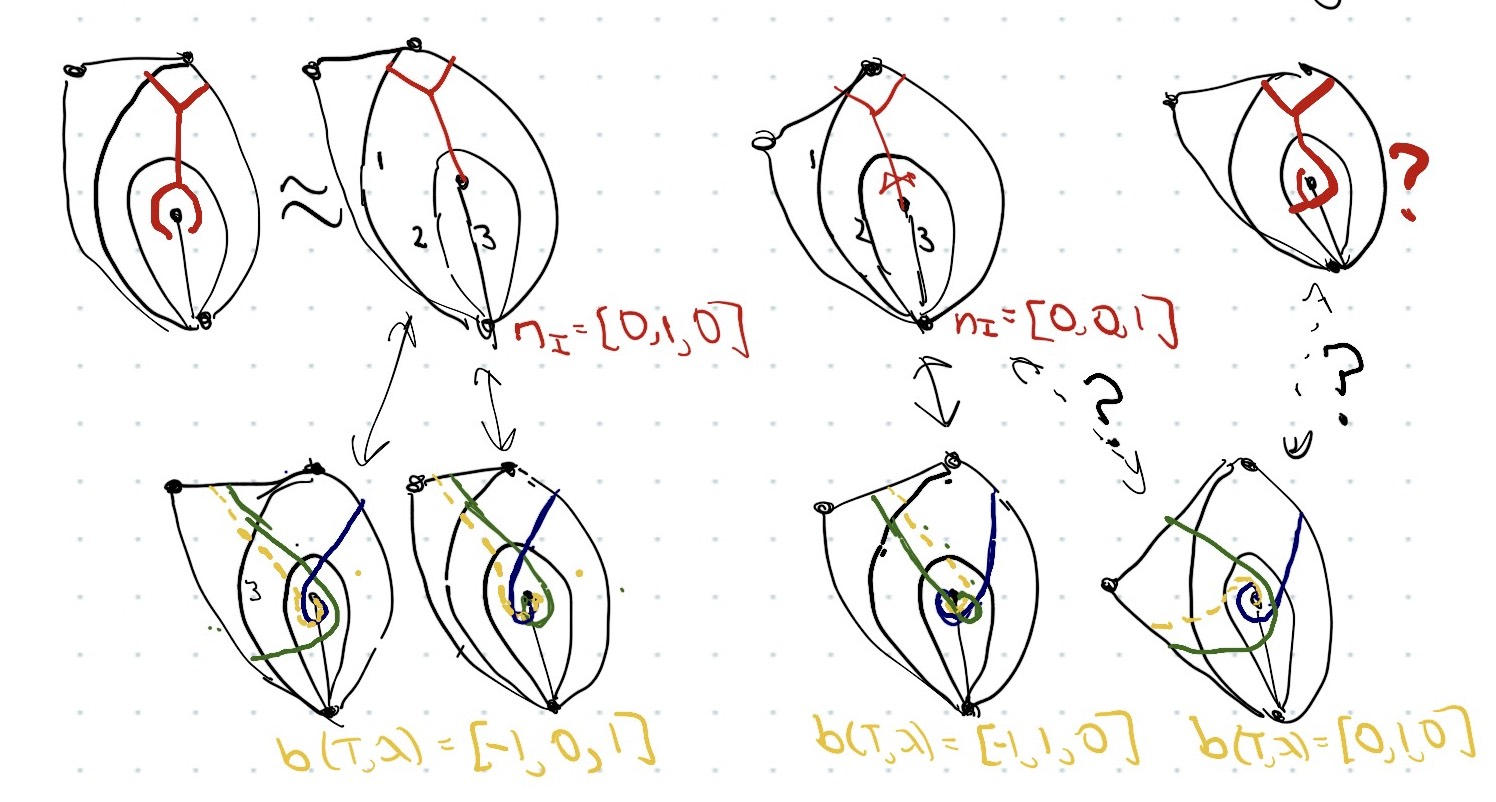
\includegraphics[scale=.2]{new_ibeam.jpg}
\end{remark}

\begin{figure}
\caption{Some simple examples}
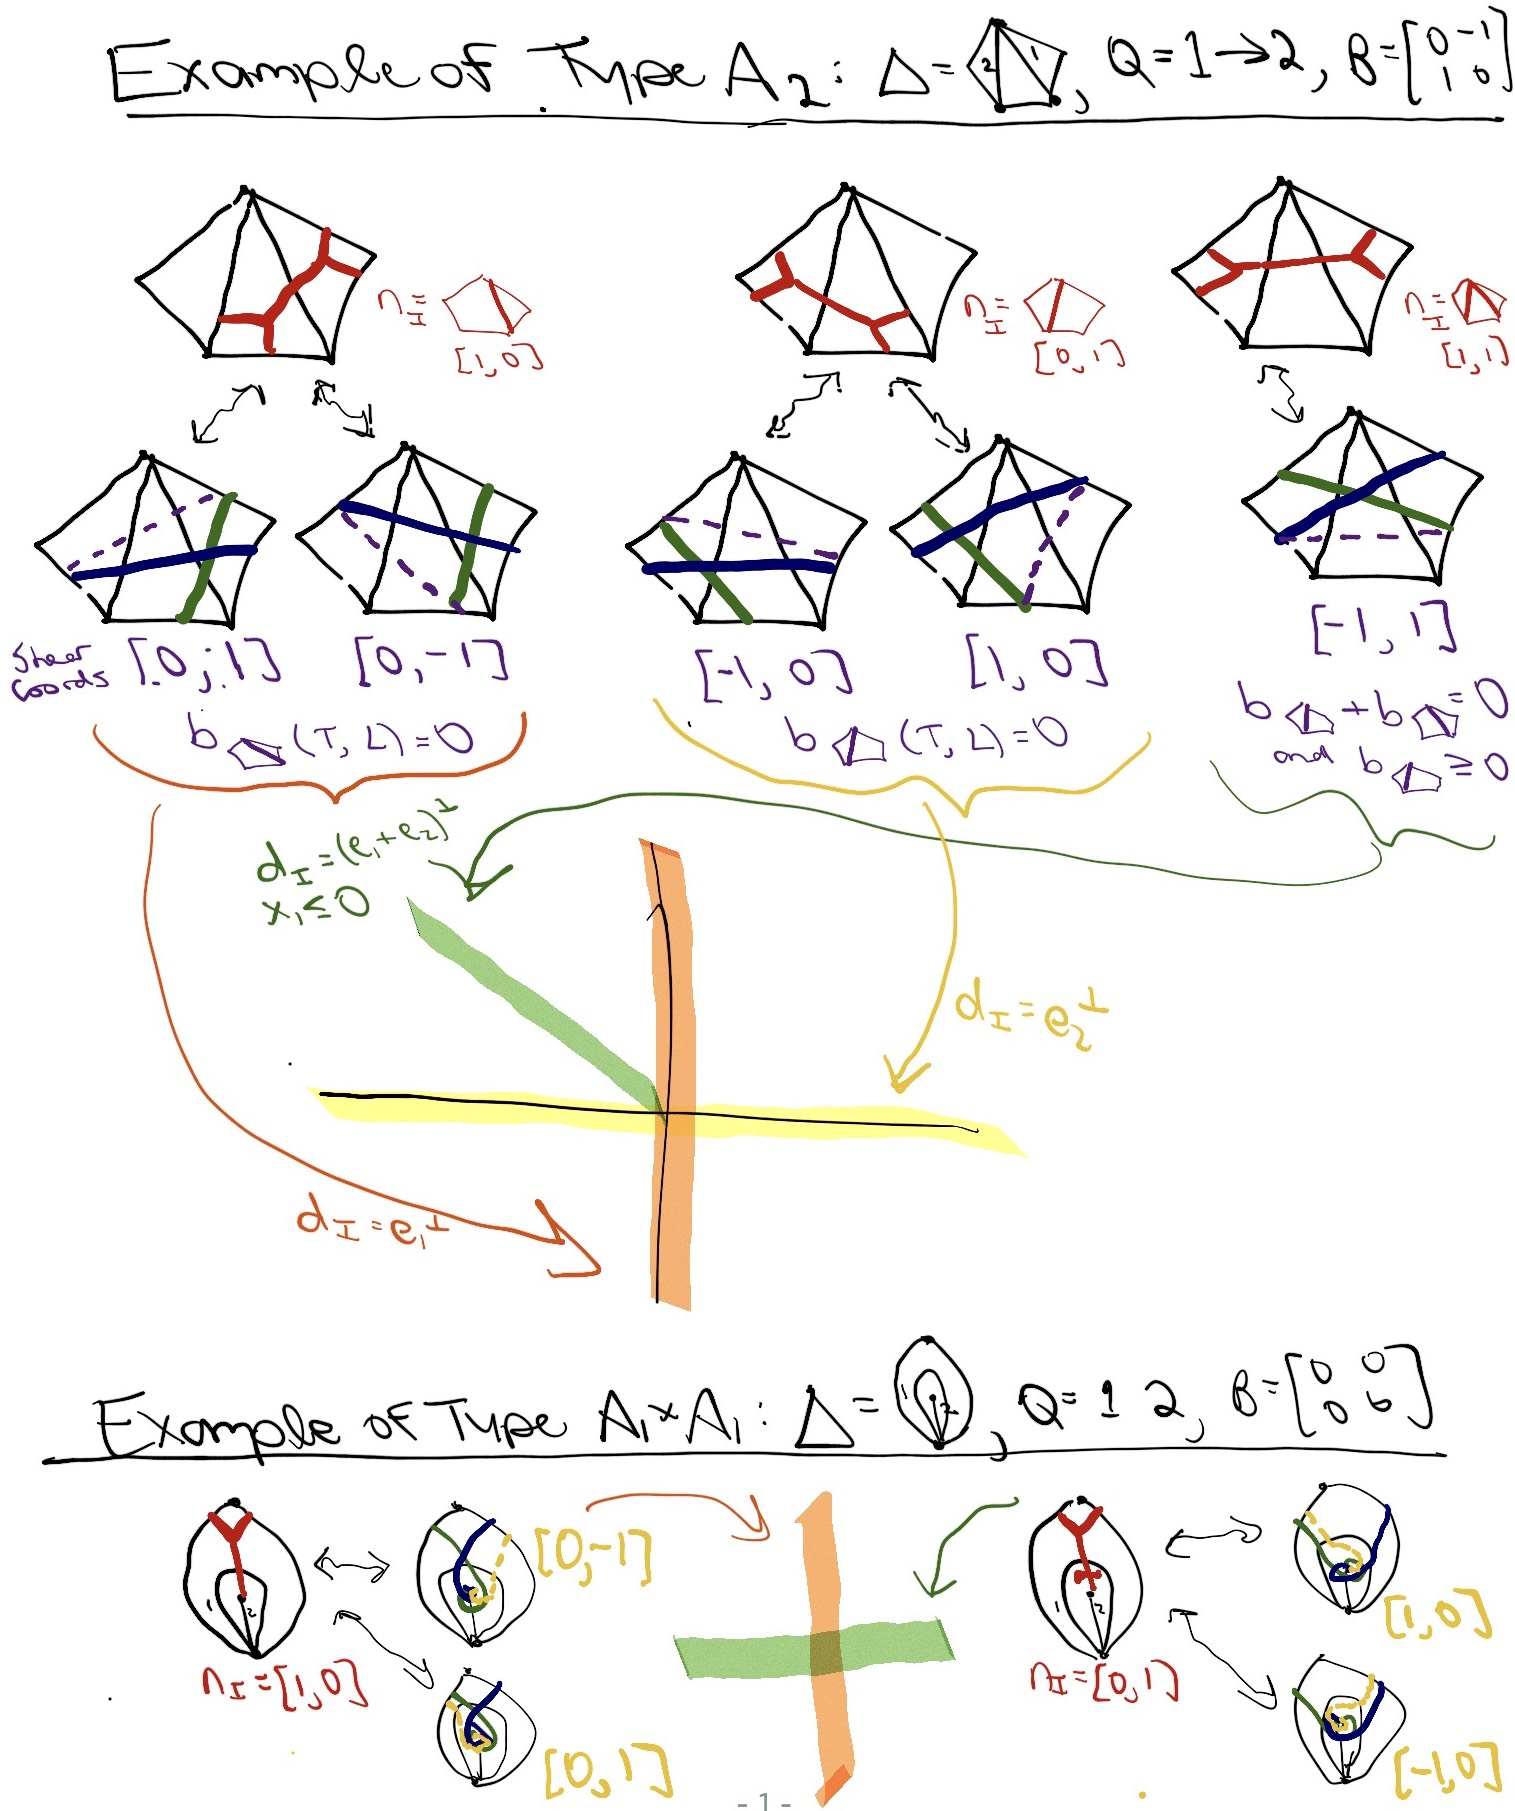
\includegraphics[scale=.25]{ibeam_examples.jpg}
\end{figure}

\begin{thebibliography}{27}
\bibitem{GHKK}
M. Gross, P. Hacking, S. Keel, and M. Kontsevich,
\textit{Canonical bases for cluster algebras.}
Preprint, 2014. \texttt{arXiv:1411.1394}

\bibitem{unisurface}
N. Reading,
\textit{Universal geometric cluster algebras from surfaces. }
Trans. Amer. Math. Soc. \textbf{366} no. 12 (2014), 6647--6685.

\end{thebibliography}

\newpage

\section{A possible alternative to I-beams and joints}

\begin{definition}
Given a triangulation $\Delta$ of unpunctured\margin[GM]{I haven't attempted punctured surfaces yet.} $(\S,\M)$, a \newword{barricade} $B$ in $\Delta$ is given by a topological graph embedded in $\S$, such that, when restricted to the neighborhood of a triangle in $\Delta$, the connected components are isotopic to one of the pictures in Figure \ref{fig: local barricade}.
%\begin{itemize}
%	\item each degree $1$ vertex lie in the interiors of arcs of $\Delta$ (or in punctures), and
%	\item each degree $3$ vertex lies in the interior of a triangle and the adjacent edges 
%\end{itemize}
\end{definition}

\begin{figure}[h!t]
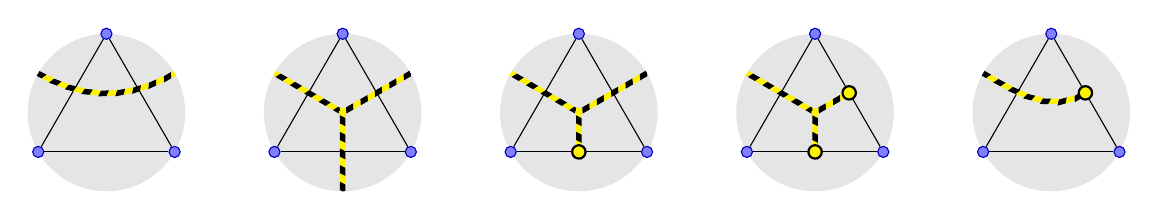
\begin{tikzpicture}[scale=1]
\begin{scope}[xshift=0cm]
	\path[fill=black!10] (0,0) circle (1);
	\node[marked] (1) at (90:1) {};
	\node[marked] (2) at (-30:1) {};
	\node[marked] (3) at (210:1) {};
	\draw (1) to node[below] {} (2);
	\draw (2) to node[below] {} (3);
	\draw (3) to node[below] {} (1);
	\clip (0,0) circle (1);
	\draw[barricade,out=210,in=-30] (30:1) to (150:1);
\end{scope}
\begin{scope}[xshift=3cm]
	\path[fill=black!10] (0,0) circle (1);
	\node[marked] (1) at (90:1) {};
	\node[marked] (2) at (-30:1) {};
	\node[marked] (3) at (210:1) {};
	\draw (1) to node[below] {} (2);
	\draw (2) to node[below] {} (3);
	\draw (3) to node[below] {} (1);
	\clip (0,0) circle (1);
	\draw[barricade] (150:1) to (0,0);
	\draw[barricade] (0,0) to (30:1);
	\draw[barricade] (0,0) to (270:1);
\end{scope}
\begin{scope}[xshift=6cm]
	\path[fill=black!10] (0,0) circle (1);
	\node[marked] (1) at (90:1) {};
	\node[marked] (2) at (-30:1) {};
	\node[marked] (3) at (210:1) {};
	\draw (1) to node[below] {} (2);
	\draw (2) to node[below] {} (3);
	\draw (3) to node[below] {} (1);
	\clip (0,0) circle (1);
	\draw[barricade] (150:1) to (0,0);
	\draw[barricade] (0,0) to (30:1);
	\draw[barricade] (0,0) to (270:.5);
	\node[barricade vertex] (b) at (270:.5) {};
\end{scope}
\begin{scope}[xshift=9cm]
	\path[fill=black!10] (0,0) circle (1);
	\node[marked] (1) at (90:1) {};
	\node[marked] (2) at (-30:1) {};
	\node[marked] (3) at (210:1) {};
	\draw (1) to node[below] {} (2);
	\draw (2) to node[below] {} (3);
	\draw (3) to node[below] {} (1);
	\clip (0,0) circle (1);
	\draw[barricade] (150:1) to (0,0);
	\draw[barricade] (0,0) to (30:.5);
	\draw[barricade] (0,0) to (270:.5);
	\node[barricade vertex] (a) at (30:.5) {};
	\node[barricade vertex] (b) at (270:.5) {};
\end{scope}
\begin{scope}[xshift=12cm]
	\path[fill=black!10] (0,0) circle (1);
	\node[marked] (1) at (90:1) {};
	\node[marked] (2) at (-30:1) {};
	\node[marked] (3) at (210:1) {};
	\draw (1) to node[below] {} (2);
	\draw (2) to node[below] {} (3);
	\draw (3) to node[below] {} (1);
	\clip (0,0) circle (1);
	\draw[barricade,out=210,in=-30] (30:.5) to (150:1);
	\node[barricade vertex] (a) at (30:.5) {};
\end{scope}
\end{tikzpicture}
\caption{Local pictures of barricades (up to rotation and reflection)}
\label{fig: local barricade}
\end{figure}

A \newword{long leaf}\margin[GM]{I can't decide if we want to allow long leaves in the definition. They make the proof of Prop. \ref{prop: inequalities} easier, but they don't appear in barricades related to the scattering diagram.} is a leaf whose adjacent vertex is not in the adjacent triangle (the fifth local picture in Figure 
\ref{fig: local barricade}).
Barricades are considered up to isotopy within the set of barricades (so leaves must remain on arcs in $\Delta$). 
A measured lamination $\mu$ is \newword{compatible} with a barricade $B$ if there is are equivalent $\mu'$ and $B'$ such that $\mu'$ intersects $\Delta$ minimally and $\mu'$ and $B'$ do not intersect.%\margin[GM]{`Compatible' is a bit fiddly to define, since we need to be able to move the barricade around, but not 

\begin{prop}\label{prop: inequalities}
Given a barricade $B$, a measured lamination $\mu$ is compatible with $B$ iff the following inequalities hold.
\begin{itemize}
	\item For each path in $B$ which begins with a right turn and ends with a left turn,
	\[ S_{1}(\mu) + S_{2}(\mu) + ... + S_{n}(\mu) \geq 0\]
	where $S_1, S_2,...,S_n$ are the shear coordinates of the arcs in $\Delta$ crossed by $P$.
	\item For each path in $B$ which begins with a left turn and ends with a right turn, 
	\[ S_{1}(\mu) + S_{2}(\mu) + ... + S_{n}(\mu) \leq 0\]
	where $S_1, S_2,...,S_n$ are the shear coordinates of the arcs in $\Delta$ crossed by $P$.
	\item For each cycle in $B$, 
	\[ S_{1}(\mu) + S_{2}(\mu) + ... + S_{n}(\mu) = 0\]
	where $S_1, S_2,...,S_n$ are the shear coordinates of the arcs in $\Delta$ crossed by $P$.
\end{itemize}
\end{prop}

\begin{corollary}
As a subset of $\mathbb{R}^\Delta$, the set of measured laminations which are compatible with $B$ is a closed cone. \end{corollary}

\begin{definition}
The \newword{codimension} of a barricade is the codimension of (the span of) the compatible cone. A barricade is \newword{minimal} if it has no sub-barricades of the same codimension.
\end{definition}

Easy observation: a minimal barricade has no long leaves, since they can be cut off without increasing the codimension.

%If $B$ has no loops, the span of the compatible cone has codimension equal to the number of edges in $B$ whose endpoints are degree $3$ vertices.

\begin{prop}[I-beams]
The minimal barricades of codimension $1$ are:
\begin{itemize}
	\item Trees with $4$ leaves (none long).
	%which are locally isomorphic to the pictures in Figure \ref{fig: local I-beams}.
	\item A non-shielding cycle with $0$ leaves.
\end{itemize}
\end{prop}

%\begin{definition}
%Given an (ordinary, untagged) triangulation $\Delta$ of $(\S,\M)$, an \newword{I-beam} is a graph $I$ embedded in $\S$, such that, when restricted to the neighborhood of a triangle in $\Delta$, the connected components are isotopic to one of pictures in Figure \ref{fig: local I-beams}.
%\end{definition}

%\begin{figure}[h!t]
%\begin{tikzpicture}[scale=1]
%\begin{scope}[xshift=0cm]
%	\draw[fill=black!10, dashed] (0,0) circle (1);
%	\node[marked] (1) at (90:1) {};
%	\node[marked] (2) at (-30:1) {};
%	\node[marked] (3) at (210:1) {};
%	\draw (1) to node[below] {} (2);
%	\draw (2) to node[below] {} (3);
%	\draw (3) to node[below] {} (1);
%	\draw[red,out=210,in=-30] (30:1) to (150:1);
%\end{scope}
%\begin{scope}[xshift=3cm]
%	\draw[fill=black!10, dashed] (0,0) circle (1);
%	\node[marked] (1) at (90:1) {};
%	\node[marked] (2) at (-30:1) {};
%	\node[marked] (3) at (210:1) {};
%	\draw (1) to node[below] {} (2);
%	\draw (2) to node[below] {} (3);
%	\draw (3) to node[below] {} (1);
%	\node[inner sep=0.5mm,circle,draw=red] (a) at (30:.5) {};
%	\node[inner sep=0.5mm,circle,draw=red] (b) at (270:.5) {};
%	\draw[red] (150:1) to (0,0);
%	\draw[red] (0,0) to (a);
%	\draw[red] (0,0) to (b);
%\end{scope}
%%\begin{scope}[xshift=6cm]
%%	\draw[fill=black!10, dashed] (0,0) circle (1);
%%	\node[marked] (1) at (90:1) {};
%%	\node[marked] (2) at (270:1) {};
%%	\node[marked] (3) at (0,0) {};
%%	\draw[out=-15,in=15] (1) to (2);
%%	\draw[out=195,in=165] (1) to (2);
%%	\draw[out=-60,in=60] (1) to (3);
%%	\draw[out=-120,in=120] (1) to (3);
%%	\draw[red] (3) to (0,-.5);
%%	\draw[red,out=-30,in=210] (0,.-.5) to (0:1);
%%	\draw[red,out=210,in=-30] (0,.-.5) to (180:1);
%%\end{scope}
%%\begin{scope}[xshift=9cm]
%%	\draw[fill=black!10, dashed] (0,0) circle (1);
%%	\node[marked] (1) at (90:1) {};
%%	\node[marked] (2) at (270:1) {};
%%	\node[marked] (3) at (0,0) {};
%%	\draw[out=-15,in=15] (1) to (2);
%%	\draw[out=195,in=165] (1) to (2);
%%	\draw[out=-60,in=60] (1) to (3);
%%	\draw[out=-120,in=120] (1) to (3);
%%	\draw[red] (3) to (0,-.5);
%%	\draw[red,out=-30,in=210] (0,.-.5) to (0:1);
%%	\draw[red,out=210,in=-30] (0,.-.5) to (180:1);
%%\end{scope}
%\end{tikzpicture}
%\caption{Local pictures of I-beams (no punctures)}
%\label{fig: local I-beams}
%\end{figure}

\begin{prop}[Joints]
The minimal barricades of codimension $2$ are:
\begin{itemize}
	\item Trees with $5$ leaves (none long).
	\item A non-shielding cycle with $2$ leaves (none long).
	\item Disjoint unions of $2$ minimal barricades of codimension $1$.
\end{itemize}
\end{prop}

\begin{thm}
The scattering diagram of $(\S,\M)$ in $\mathbb{R}^\Delta$ has a wall for each minimal barricade of codimension $1$ (supported on the compatible cone), and a joint for each minimal barricade of codimension $2$ (supported on the compatible cone).
\end{thm}

%\newpage

\section{Proof of Proposition \ref{prop: inequalities}}

Let us collectively refer to the inequalities in Proposition \ref{prop: inequalities} as the \newword{compatibility inequalities} for $B$ and $\mu$. 

A barricade is \newword{simple} if it is connected and has no degree $3$ vertices. We start by proving a stronger version of Proposition \ref{prop: inequalities} in the case of a simple barricades.

\begin{lemma}\label{lemma: simplebarricade}
Let $B$ be a simple barricade in $\Delta$. A measured lamination $\mu$ is compatible with $B$ iff it satisfies the compatibility inequalities. 

Furthermore, if the longest path in $B$ begins with a right turn and ends with a left turn, then 
\[ S_1(\mu) + S_2(\mu) + ... + S_n(\mu)\]
is the total measure of $B$ in $\mu$. Similarly, if the longest path in $B$ begins with a left turn and ends with a right turn, then 
\[ -S_1(\mu) - S_2(\mu) - ... - S_n(\mu)\]
\end{lemma}

\begin{proof}[Proof idea]
Induction, I hope. I don't know about loops, though.
\end{proof}

\begin{lemma}\label{lemma: simplesub}
A measured lamination $\mu$ is compatible with a barricade $B$ iff $\mu$ is compatible with every simple sub-barricade of $B$.
\end{lemma}

\begin{proof}[Proof idea]
If they are incompatible, there should be some unmarked curve that is crossed.
\end{proof}

\begin{proof}[Proof of Proposition \ref{prop: inequalities}]
Assume $\mu$ is compatible with $B$. For any path or cycle in $B$, there is a simple sub-barricade $B'$ containing that path or cycle which is also compatible with $\mu$, and so the associated compatibility inequality holds by Lemma \ref{lemma: simplebarricade}.

Assume the compatibility inequalities hold for $\mu$ and $B$. Then they also hold for any simple sub-barricade of $B$, and so by Lemma \ref{lemma: simplebarricade} $\mu$ is compatible with each of them. By Lemma \ref{lemma: simplesub}, $\mu$ is compatible with $B$.
\end{proof}

\section{Minimal barricades}

\begin{conj}
The codimension of a barricade $B$ is 
\begin{align*}
\#&\text{ of edges in $B$ with a branch at each endpoint} \\
&+ \#\text{ of loops (i.e. cycles without branches)} \\
&+ \text{total genus of components of $\S\smallsetminus B$ that don't contain marked points}\\
\end{align*}
\end{conj}


\end{document}  